\documentclass[letterpaper]{article}
\usepackage{graphicx}
\usepackage{multicol}
\graphicspath{ {./} }

\title{
    Speechify - STP and Value Proposition\\
    \begin{large}
        Winter 2021 - COMM 302 - Assignment 2
    \end{large}
}
\author{Jamie Won - 20113217}

\begin{document}
\maketitle
\tableofcontents
\cleardoublepage

\section{Segmentation}
    Four potential market segments were identified for Speechify: AudioBook Companies, Video Editors, and Teachers/Instructors. These market segments will be described further in the sections below, as well as their need for Speechify. Discussion on the selection of the market segment is in the subsequent section, Targeting.
    \subsection{Audiobook Companies}
        An audiobook company is defined as an individual or organization that wishes to enhance existing aural material with music, where, the material can be a book, article, document or any other written content. There is a trend in audiobooks towards those with background music and those that do tend to sell better [5]. Audiobook companies typically attempt to increase their profit margin and increasing sales is one way to do so.
    \subsection{Video Editors}
        A video editor is defined as anyone who enhances videos manually. These people range from students editting a video for a school project, to industry professionals who select and put together movie soundtracks. However, background music is not the only task of a video editor, and they want to be more efficient so that they can make better use of their time. Thus, they are seeking for a tool that is integrates well with existing tools and is not too different structurally.
    \subsection{Teachers/Instructors}
        A teacher or instructor is defined as any person(s) who facilitate the transfer of knowledge and skills. These people must effectively communicate while keeping their class' interest and focus. Studies show that background music helps create a "positive classroom environment" [6]. In an age of online schooling where every class is a video, aural stimulation can be what keeps student interest. As a large portion of the teaching population is old[er], they seek something that is easy to use.
    \subsection{Content Creators}
        A content creator is defined as any person(s) who creates new digital content for the entertainment of others. Note that video editors are a subset of this category and the other two segments are not. By the definitions in the previous sections, audiobook companies are not creating new content, and teachers/instructors do so for education rather than entertainment purposes, and thus, do not fall under this category. With the advent of centralized streaming platforms, content is devalued, and creators must churn out content that is both high in quantity and quality while competing with others doing the same. They seek something that is easy to use, quick and low cost.
\section{Targeting}
    \subsection{The Target Market}
        As recommended by Bill Aulet, Speechify will seek to exploit a beachhead market. The target market segment is that of content creators. The following table details the reasoning for this choice. Where applicable, number values are rankings amongst the potential segments, with "1" denoting the best (ie largest market size, highest profitability, lowest risk) and "4" denoting the worst.
        \begin{figure}
            
            \begin{tabular} { | c | c | c | c | c | }
                \hline
                \begin{tabular}{@{}c@{}}Variable / \\Segment\end{tabular} & \begin{tabular}{@{}c@{}}Audiobook \\ Companies\end{tabular} & \begin{tabular}{@{}c@{}}Video \\ Editors\end{tabular} & \begin{tabular}{@{}c@{}}Teachers /\\Instructors\end{tabular} & \begin{tabular}{@{}c@{}}Content \\ Creators\end{tabular}\\
                \hline
                Competition & 4 & 3 & 1 & 2 \\
                \hline
                Customer Need & 4 & 1 & 3 & 2 \\
                \hline
                Fit & 3 & 2 & 4 & 1 \\
                \hline
                Funding & 2 & 3 & 1 & 4\\
                \hline
                Easily Accessible & 3 & 2 & 4 & 1\\
                \hline
                Market Growth & 4 & 3 & 2 & 1 \\
                \hline
                Profitability & 2 & 3 & 4 & 1\\
                \hline
                Protectability & 2 & 3 & 1 & 4\\
                \hline
                Risk & 3 & 2 & 1 & 4\\
                \hline
                Saturation & 4 & 2 & 3 & 1\\
                \hline
                Size & 3 & 2 & 4 & 1\\
                \hline
                Total Scores & 30 & 26 & 28 & 22\\
                \hline
            \end{tabular}
            \caption{An evaluation matrix for the different market segments}
        \end{figure}
        \par
        It should be noted that all variables are given the same weight. The reason for this is, after, analysis, all the variables appear to be related to each other, and any discrepancy in their weights cancel out. For example, consider protectability, risk and teachers/instructors. The education market is a riskier venture as institutions must adhere to a plethora of laws. On the other hand, they usually sign contracts for SAAS products, and thus are highly protectable. From the matrix, it is clear that content creators are the most viable market segment. The following section details further analysis of the claim.
    \subsection{Further Analysis}
        \subsubsection{Company Resources}
            The biggest contraint on resources is money. As a startup, it is unlikely Speechify will have a large development team, but as a member of the SAAS industry, it needs developers. However, having a dedicated developer (or two) will allow for the creation of an MVP. If there is a developer on the co-founding team, less resources will be needed (salary). Capital can be earned by applying to grants and [hopefully] winning pitch competitions, and a strong publicity/marketing team (members of the cofounding team) will be key in doing so.
        \subsubsection{Product and Market Variability}
            For the target market, either the freemium or free for personal use would be ideal. Independent content creators often have little resources themselves, and if they develop a reliance on Speechify, will hopefully look to use its additional capabilities. If they ever "blow up" then they will have capital to spend and will need the extra features. Larger content creators, that is, companies or people with a sizable number of followers also fall into this category.
        \subsubsection{Competitor's Marketing Strategies}
            For this segment, there are currently no competitors. Should there be new entrants, Speechify will already have a foothold in the market and use its name to attract more clients.
        
    \subsection{Customer Personas}
        \subsubsection{Abigail "Videos are so cool" Summers (The Kid)}
            \begin{multicols}{2}
                
\includegraphics[width=4.5cm, height=5cm]{girl}
                \begin{large}
                    About Abigail:
                \end{large}
                \begin{itemize}
                    \item Age: 16 years old
                    \item Education: Currently in primary school
                    \item Occupation: Student \& volunteer video editor
                    % \item Relationship Status: Single, but looking for a boyfriend
                    \item Family Status: Two parents (married) and one sibling
                \end{itemize}
            \end{multicols}
            \begin{multicols}{2}
                \begin{large}
                    Behaviour
                \end{large}
                \begin{itemize}
                    \item Always chooses the video option for creative projects
                    \item A go-getter, willing to do extra work to get the results she wants
                    \item Is the friend who always has  a story to tell (she makes them up when she doesn't have any new ones)
                \end{itemize}
                \begin{large}
                    Needs, Wants and Expectations
                \end{large}
                \begin{itemize}
                    \item Needs a tool that is easy to use and works quickly
                    \item Wants to do well in school, hang out with friends, go into film
                    \item Expects to get into a good university and spend the rest of her life creating new things
                \end{itemize}
            \end{multicols}
            Abigail has \emph{limited to moderate} video editting skills (depending on who is asked). Her main concern is that video editting \emph{takes a long time}. When she grows up, she will continue to use Speechify and desire more of its features!
        \subsubsection{Tony "Imma make it big" Banners (The Creator)}
        \begin{multicols}{2}
            
\includegraphics[width=5cm, height=5cm]{boy}
            \begin{large}
                About Tony:
            \end{large}
            \begin{itemize}
                \item Age: 22 years old
                \item Education: University Student
                \item Relationship Status: Girlfriend of 2 years
                \item Housing Status: Shares a flat with 2 classmates
                \item Occupation: Part-time TikTok star
            \end{itemize}
        \end{multicols}
        \begin{multicols}{2}
            \begin{large}
                Behaviour
            \end{large}
            \begin{itemize}
                \item Excitable, a good speaker and very creative
                \item Tries to do work quickly, procrastinates sometimes, but is very good at cramming
                \item Willing to put in extra effort if it'll help in the long run
            \end{itemize}
            \begin{large}
                Needs, Wants and Expectations
            \end{large}
            \begin{itemize}
                \item Needs a tool that increases efficiency and is free, or low cost
                \item Wants to "blow up" and get his content to more viewers
                \item Expects it to be tough, that there will be competition, but will persevere as long as he can afford it
            \end{itemize}
        \end{multicols}
        Tony has \emph{familiarity} with video editting software, but the tools he needs to be more efficient are \emph{expensive}. There are so many others trying for stardom - he needs to produce \emph{more and better} content. If Tony makes it big, he'll want more of Speechify's features. Until them, he will use a minimal or middle tier plan.

    \subsection{Total Addressable Market}
    Abigails become Tonys in the future. There were 1.4 M Canadian university students in 2019 and likely 50000 of them are Tonys [3]. The global content SAAS penetration rate has increased from 12-24\% from 2015-2020 [4]. Assuming it takes a year for production, for a conservative estimate, it shall be assumed that the penetration rate for 2022 remains at 24%
    \[ Market\: volume = Number\: of\: target\: customers\: x\: Penetration\: rate \]
    \[ Market\: volume = 50 000\: x\: 0.24 = 12 000 \]
    \[ Market\: value = Market\: volume\: x\: Average\: value \]
    \[ Market\: value = 12 000\: x\: 60 = 720 000 \]
    Note that this assumes a monthly fee of \$5 and these people buy for the entire year. It is an extremely conservative estimate, not factoring in the ones who purchase the elite tier of the product. Thus, the total addressable market is about 720 000 for 2022.
    \par
    Over the next years, Speechify will transition to larger institutions instead of individual content creators and as such, the market will change.
\section{Value Proposition}
    \subsection{Value Proposition Statement}
        Speechify helps creators make content that is both high in quantity and quality through a easy-to-use, beautiful interface that quickly enhances audio files with appropriate music, reducing the time spent on each piece by up to 80\%.
    \subsection{Value Proposition Canvas}
        \begin{tabular} { | p{2cm} | p{3.25cm} | p{3.25cm}| p{1.75cm} |}
            \hline
             & \textbf{Value Proposition} & \textbf{Customer Segment} & \\
            \hline
            \textbf{Products and Services} 
            & Software that performs sentimental analysis on an audio clip and enhances it with music
            & Content Creators; Video Editors
            & \textbf{Customer Jobs}\\
            \hline
            \textbf{Gain Creators} 
            & Allows users to produce more through a pretty, usable interface by saving time 
            & Produce more content, faster and better; an aesthetic, easy-to-use interface
            & \textbf{Gains} \\
            \hline
            \textbf{Pain Relievers} 
            & Lessens time needed to edit videos; Freemium model
            & Video editting is very slow, especially finding and concatenating audio files; SAAS is expensive
            & \textbf{Pains} \\
            \hline
        \end{tabular}
\section{Positioning}
    \subsection{Positioning Statement}
    To young content creators looking to "make it big", Speechify is the software service that saves the most time because it nearly erases the time needed to enhance video soundtracks.
    \subsection{Positioning Map}
    It should be noted that this is an untapped market - there are no competitors. While there are services that help with video editting, and others that let one generate music, there are none that do so based on the content and combine the files, with transitions, smoothly. A few video editting softwares are included in the positioning map, wher as these also help creators save time.
    \begin{figure}
        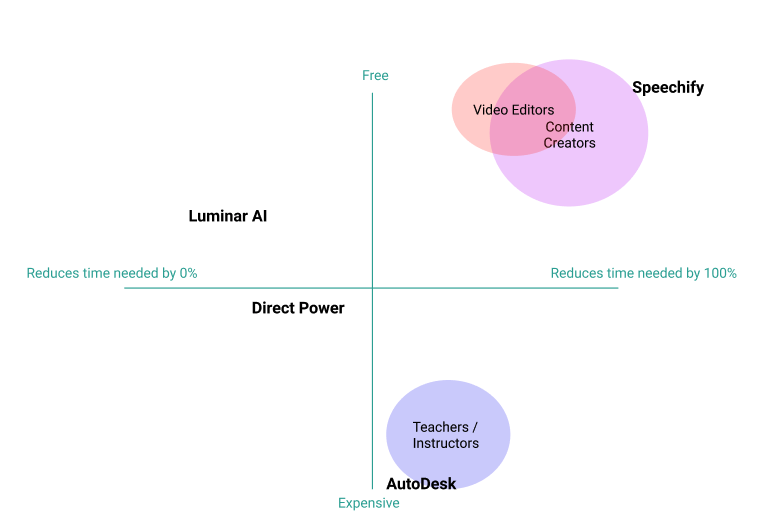
\includegraphics[width=11cm]{PositioningMap}
        \caption{Speechify's Positioning Map}
    \end{figure}
\cleardoublepage
\section{References}
\begin{itemize}
    \item Aulet, B. (2013). Disciplined Entrepreneurship: 24 Steps to a Successful Startup (1st ed.). Wiley.
    \item C. (2020, June 3). How long does it take to edit a video? How much work is running a youtube channel? Changing Lanes. https://changinglanesrv.com/ufaqs/how-long-does-it-take-to-edit-a-video-how-much-work-is-running-a-youtube-channel/.
    \item Facts and stats. (2018, July 31). Universities Canada. https://www.univcan.ca/universities/facts-and-stats/
    \item Kozlowski, M. (2020, June 21). Audiobook Trends and Statistics for 2020. Good E-Reader. https://goodereader.com/blog/audiobooks/audiobook-trends-and-statistics-for-2020
    \item Mars Discovery District. (2020, November 18). Estimating market size | Business \& Marketing Planning | Startups. MaRS Startup Toolkit. https://learn.marsdd.com/article/how-to-estimate-market-size-business-and-marketing-planning-for-startups/
    \item Olóndriz, P. (2020, December 15). Music for Audiobooks. Legis Music. https://legismusic.com/music-audiobooks/
    \item Statista. (2021, January 12). Global SaaS penetration rate 2015-2020, by application. https://www.statista.com/statistics/782240/worldwide-software-as-a-service-applications-penetration-rate/
    \item U. (n.d.-a). 100+ Girls Pictures | Download Free Girl Photos on. Unsplash. Retrieved January 31, 2021, from https://unsplash.com/s/photos/girl
    \item U. (n.d.-b). 500+ Boy Photos [HD] | Download Free Images On. Unsplash. Retrieved January 31, 2021, from https://unsplash.com/s/photos/boy
\end{itemize}

\end{document}